Wie bereits im Kapitel 3.1.2 beschrieben, muss durch die Verwendung von OSS der konkrete Prozess innerhalb des HAF-Projektes angepasst werden. 

Die erste notwendige Anpassung erfolgt mittels einer Überprüfung der verwendeten Lizenzmodelle basierend auf einer manuellen Checkliste durch die entsprechenden Entwickler.  

Durch das strukturierte und mehrmalige Arbeiten mit einer manuellen Checkliste entsteht eine Routine für das Entwicklerteam innerhalb des gesamten Softwareentwicklungsprozesses. 

Der Einsatz schafft Effizenz und eine Zeitersparnis, da nur das Lizenzmodell betrachetet wird, was in diesem Moment verwendet werden möchte. 

Dieser Schritt entspricht zwar nicht der gängigen DevOps-Kultur einen möglichst hohen Grad an Automatisierung zu erlangen, jedoch kann bereits durch einen kurzen manuellen Check 'gefährliche' und 'ungefährliche' Lizenzmodelle voneinander unterschieden werden bevor eine langwierige Entwicklung stattfindet. 

Ferner ist an diesem anfänglichen Entwicklungszeitpunkt die Überprüfung mittels einer automatisierten Checkliste bedenklich, da mit der Software zunächst vorrangig expermentiert wird und eine vollständige Integration in die bestehende Anwendung somit nicht feststeht.

Andernfalls müsste jede heruntergeladene OSS direkt in das Softwareentwicklungsprozess integriert werden, um diese anschließend automatisiert überprüfen zu lassen.

Die Folgen wären ein Verlust von wichtigen Ressourcen, Effizenz und Zeit.

Ziel des Einsatzes der manuellen Checkliste ist es, sowohl die technische als auch juristische Faktoren bei der Verwendung von OSS zu berücksichtigen und ein gemeinsames Verständnis zu erreichen.

Innerhalb der kommerziellen Softwareentwicklung stellt dies eine große Herausforderung dar.

Softwarearchitekten haben oftmals eine starke funktionale und strukurelle Sichtweise und wenig Affinität zu Lizenztexten. 

Juristen hingegen haben ein Verständnis für Lizenzrecht, allerdings fällt es ihnen schwer, die tatsächliche technische Ausprägung einer Softwarekomponente rechtlich zu intepretieren. 

Die unten stehende manuelle Checkliste war bereits innerhalb der msg systems ag erstellt worden und im Rahmen dieser Arbeit auf das Problemfeld erweitert und angepasst.
%Hier Fußzeile zu dem OSS-Guide von Ralf und Navina 

\paragraph{Use Types}

Zunächst werden die 'Use Types' also die unterschiedlichen Nutzungarten erläutert. 

Diese geben Auskunft darüber, welche Bedinungen zu den jeweiligen Nutzungsarten erfüllt sein müssen. 

So enthalten einige OSS-Lizenzen beispielsweise die Klausel, dass Modifikationen des Quellcodes nur gestattet sind, wenn diese 'unter derselben OSS-Lizenz wieder allen zur Verfügung gestellt werden.'

Die vorgestellten Szenarien dienen als jeweilige Ausgangssituation, während die Nutzungsarten die jeweilige Verwendung detailliert beschreiben. 

\subparagraph{Auflistung der Nutzungsarten}

Insgesamt gibt es 14 zu beachtende Nutzungsarten.

Diese wurden in sieben verschiedene Kategorien unterteilt: Format (format), Abhängigkeit (dependency), Auslieferung (delivery), Einsatz (usage), Kommunikation (communication), Bündelung (bundling) und Artifakte (artifact). 

%Frage Daniel: kann ich die hauptsächlichen Überschriften auf englisch lassen,oder soll ich alles auf deutsch übersetzten ?????

\begin{landscape}
\begin{longtable}[h]{|l|c|c||c|c|c|}
    Use Types & Erklärung & Beispiel & SZ 1 & SZ 2 & SZ 3 \\
    \hline
    \hline
    format: source & \parbox{6cm}{Komponente wird im unverfälschten Quellformat geliefert} & WEB-INF/jquery.js & \checkmark & \checkmark & \checkmark \\
    \hline
    format: compiled & \parbox{6cm}{Komponente wird in kompiliertem Format bereitgestellt} & com/example/foo.class & - & \checkmark & \checkmark \\
    \hline
    dependency: optional  & \parbox{6cm}{Komponente wird bei Bedarf geladen, und das Produkt würde vernünftigerweise ohne sie funktionieren} & JDBC driver & \checkmark & - & - \\
    \hline
    dependency: mandatory & \parbox{6cm}{Komponente wird dynamisch/statisch geladen/verlinkt und das Produkt funktioniert nicht ohne sie} & Hibernate ORM & - & \checkmark & \checkmark \\
    \hline
    delivery: internal & \parbox{6cm}{Komponente wird intern verwendet, ohne dass sie an andere Rechtssubjekte weitergegeben wird (z. B. zeitlich begrenzte Komponenten)} & Gradle/Ant/Maven & \checkmark & - & - \\
    \hline
    delivery: distributed & \parbox{6cm}{Komponente wird an andere Rechtssubjekte verteilt (z.B. Laufzeitkomponenten)} & lib/example-1.2.3.jar & - & \checkmark & \checkmark \\
    \hline
    usage: local-call & \parbox{6cm}{Komponente (über Produkt) wird lokal zur Ausführung aufgerufen} & C:\textbackslash Applications\textbackslash  Example\textbackslash example.jar & - & \checkmark & \checkmark \\
    \hline
    usage: remote-call & \parbox{6cm}{Komponente (über das Produkt) wird remote zur Ausführung aufgerufen (SaaS)} & service.beispiel.com:1234 & - & - & - \\
    \hline
    communication: process & \parbox{6cm}{Komponente wird aufgerufen von Produkt über direkten prozessinternen Mechanismus (Funktionsaufruf, Dispatch-Tabelle, usw.)} & component\_function() & \checkmark & \checkmark & \checkmark \\
    \hline
    communication: system & \parbox{6cm}{Komponente wird vom Produkt über einen System-/Netzwerkdienst (Pipe, Socket, dlsym, execve usw.) aufgerufen} & /var/run/component.socket & - & - & - \\
    \hline
    bundling: standalone & \parbox{6cm}{Komponenten-Artefakte, die noch völlig eigenständig und als solche erkennbar sind} & example-1.2.3.jar & \checkmark & \checkmark & \checkmark \\
    \hline
    bundling: embedded & \parbox{6cm}{Komponentenartefakte, die in das Produkt eingebettet und/oder nicht offensichtlich erkennbar sind } & product-1.2.3.ear/example-1.2.3.jar & - & - & - \\
    \hline
    artifact: pristine & \parbox{6cm}{alle Komponenten-Artefakte sind unverändert, d.h. genau so, wie sie ursprünglich vom vorgelagerten Hersteller erhalten wurden} & example-1.2.3.jar!com/example/foo.class & \checkmark & \checkmark & - \\
    \hline
    artifact: modified & \parbox{6cm}{Komponenten-Artefakte wurden hinzugefügt/ersetzt/entfernt} & example-1.2.3.jar!com
    /example/addon.class & - & - & \checkmark \\
    \hline\hline
\end{longtable}
\end{landscape}

\paragraph{Umfang und Ausprägung der Verpflichtungen}

Je nach Nutzungsart müssen verschiedene und festgelegte Verpflichtungen innerhalb eines vorgeschriebenen Rahmens erfüllt werden oder können unter bestimmten Bedingungen ausgeschlossen werden.

Aufgrund dessen kann der Umfang der Verplichtung sich um eine Last, die der Nutzer erfüllen muss handeln oder um eine bestimmte Nutzungsart beziehen, indem einzelne Verpflichtungen erfüllt werden müssen oder die gesamte Nutzung ausgeschlossen wird. 

\subparagraph{Umfang der Verpflichtungsarten} $~$
\\

\begin{tabular}[h]{|r|c|l|}
    \hline\hline
    Verpflichtungsumfang & Zweck & Erklärung \\
    \hline\hline
    \parbox{4cm}{OBLIGATION (OBL)} & \parbox{5cm}{Eine Bedingung muss erfüllt werden, um die Lizenzbedingungen zu erfüllen} & \parbox{5cm}{Eine Lizenzvereinbarung enthält mehrere Bedingungen, die erfüllt werden müssen} \\
    \hline
    \parbox{4cm}{NOT OBLIGATION SINGLE (NOS)} & \parbox{5cm}{Eine Bedingung ist aufgrund der Nutzung ausgeschlossen} & \parbox{5cm}{Wenn eine bestimmte Nutzung nicht eingeschränkt ist, muss die Verpflichtung nicht erfüllt werden, um die Lizenzbedingungen einzuhalten} \\
    \hline
    \parbox{4cm}{NOT OBLIGATION GLOBAL (NOG)} & \parbox{5cm}{Alle Lizenzbedingungen werden aufgrund einer bestimmten Nutzungsart ausgeschlossen} & \parbox{5cm}{Einige Lizenzvereinbarungen enthalten die Aussage, dass die Lizenzbedingungen nicht gelten, wenn die Komponente auf eine bestimmte Weise verwendet wird} \\

    \hline
\end{tabular}

\subparagraph{Ausprägung einer zu erfüllenden Verpflichtung}

Im Hinblick auf die Verpflichtungen, die der Nutzer erfüllen muss, lassen sich mehrere Elemente definieren. 

Diese geben an welche Bedingungen, innerhalb einer Verpflichtung erfüllt werden müssen. 

Ziel ist es, mittels der unterschiedlichen Ausprägungen der Verpflichtung im Zusammenhang mit den jeweiligen Use Types, eine auf das Lizenzmodell abgestimmte Aufgabenliste zu erstellen, die die jeweiligen Entwickler berücksichtigen müssen. \\

\begin{tabular}[h]{|r|c|l|}
    \hline\hline
    Verpflichtungselemente & Kurzform & Erklärung \\
    \hline\hline
    \parbox{4cm}{No Liability} & NO-LIABILITY & \parbox{6cm}{Der Urheber der Komponente kann nicht für Schäden haftbar gemacht werden, die er verursacht} \\
    \hline
    \parbox{4cm}{Keep Copyright Information} & KEEP-COPYRIGHT & \parbox{6cm}{Die Copyright-Informationen des Autors der Komponente müssen beibehalten werden} \\
    \hline
    \parbox{4cm}{Provide License Text} & PROVIDE-LICENSE & \parbox{6cm}{Der Lizenztext der Komponete muss vollständig angegeben werden} \\
    \hline
    \parbox{4cm}{Provide Source Code} & PROVIDE-SOURCE & \parbox{6cm}{Der Quellcode der Komponete muss vollständig angegeben werden} \\
    \hline
    \parbox{4cm}{Advertizement Clause} & ADV-CLAUSE & \parbox{6cm}{Die Dokumentation und/oder Anwendung muss einen Hinweis auf die Komponente (und ihren Autor) enthalten} \\ 
    \hline
    \parbox{4cm}{Name Change Required} & RENAME & \parbox{6cm}{Der Name der Komponente muss geändert werden (im Falle von Änderungen und Weiterverbreitung)} \\
    \hline
    \parbox{4cm}{No Relicensing Allowed} & NO-RELICENSE & \parbox{6cm}{Die Komponente kann nicht unter einer anderen benutzerdefinierten Lizenz erneut lizenziert werden} \\
    \hline
    \parbox{4cm}{Non-Military Use Only} & CTX-NON-MIL & \parbox{6cm}{Die Komponente darf nicht in militärischen oder nuklearen Kontexten verwendet werden} \\ 
    \hline
    \parbox{4cm}{Non-Commercial Use Only} & CTX-NON-COM & \parbox{6cm}{Die Komponente darf nicht in kommerziellen Kontexten verwendet werden} \\
    \hline
    \parbox{4cm}{Weak Copyleft Effect} & COPYLEFT-STRONG & \parbox{6cm}{Die Lizenz hat einen schwachen/eingeschränkten Copyleft-Effekt} \\
    \hline
    \parbox{4cm}{Strong Copyleft Effect} & COPYLEFT-WEAK & \parbox{6cm}{Die Lizenz hat eine starke/ vollständigen Copyleft-Effekt} \\
    \hline
    \parbox{4cm}{Non OSS Definition Compliant} & NON-OSS-DEF & \parbox{6cm}{Die Lizenz enthält Bedingungen, die nicht mit der Definition von Open Source Software übereinstimmen} \\
    \hline 
    \parbox{4cm}{Other Obligations} & OTHER & \parbox{6cm}{Die Lizenz enthält beliebige andere wichtige Bedingungen, die von uns nicht modelliert/abgedeckt werden (Fallback)} \\
    \hline 

\end{tabular}

\paragraph{Manuelle beispielhafte Überprüfung von Apache 2.0}

Leere Felder zeigen an, dass die Lizenz keine Aussage über die jeweilige Verpflichtung und die entsprechende Nutzungsart macht. 

Gefüllte Felder enthalten die Kennzeichnung welche jeweilige Verpflichtung für die jewelige Nutzungsart  durchgeführt werden muss. 

Die benötigten Informationen können implizit aus dem angegebenen Lizenzauszug des Lizenzmodells hervorgehen oder wurden explizit angegeben. 

\begin{figure}[p]
    \centering
    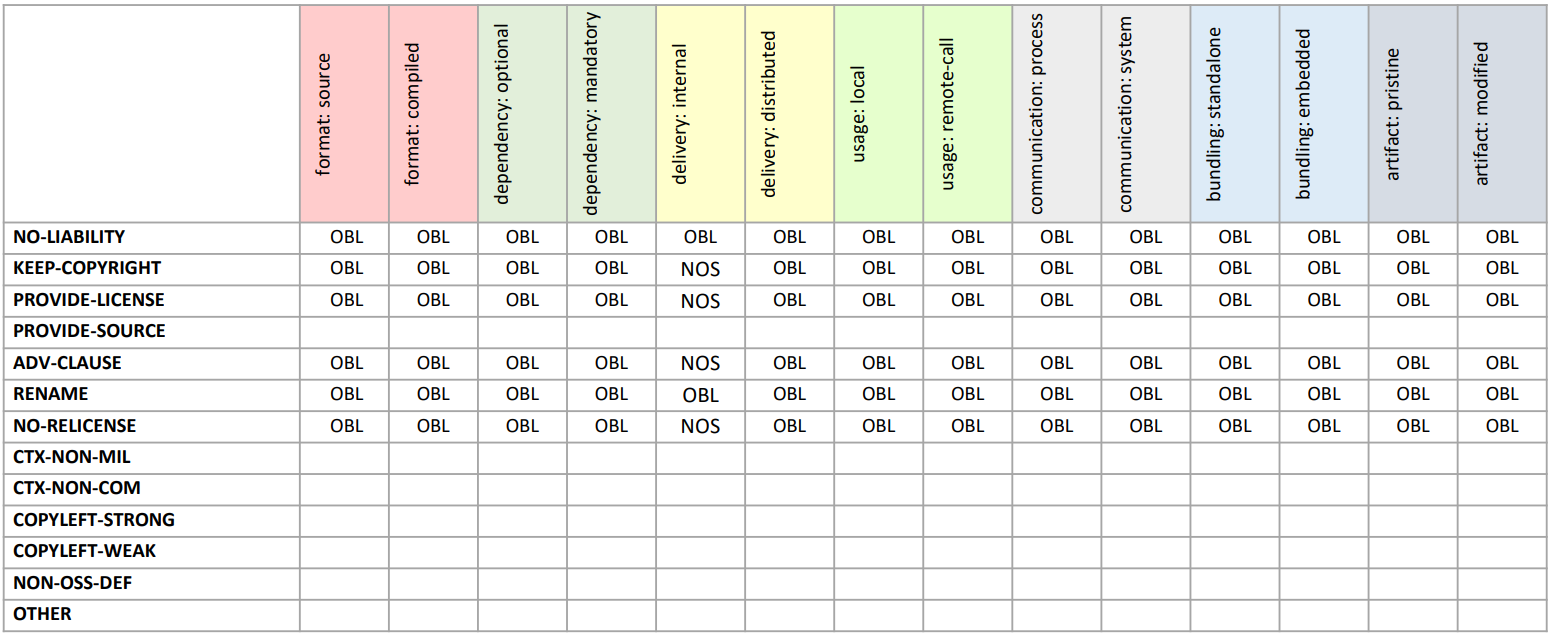
\includegraphics[angle=90, scale=0.5]{Bilder/Manuelle Checkliste.png}
\end{figure}





% Diese Checkliste wurde mit einigen Kollegen der msg systems ag zusammengestellt und entwickelt. dh Ralf und Navina erwähnen 